\documentclass[aspectratio=169,t]{beamer}

% Packages
\usepackage{amsmath,amssymb}
\usepackage{graphicx}
\usepackage{booktabs}
\usepackage{tikz}
\usetikzlibrary{shapes.geometric,arrows.meta,positioning,fit,backgrounds,calc}
\usepackage{listings}
\usepackage{xcolor}
\usepackage{multirow}

% Theme
\usetheme{Madrid}
\usecolortheme{whale}
\useinnertheme{rounded}
\setbeamertemplate{navigation symbols}{}
% Clean three-part footline with solid colored bottom boundary
\setbeamertemplate{footline}{%
  \leavevmode%
  \hbox{%
    \begin{beamercolorbox}[wd=.33\paperwidth,ht=2.5ex,dp=1.5ex,
        leftskip=6pt]{author in head/foot}%
      \usebeamerfont{author in head/foot}Pranav Bhadane%
    \end{beamercolorbox}%
    \begin{beamercolorbox}[wd=.34\paperwidth,ht=2.5ex,dp=1.5ex,center]{title in head/foot}%
      \usebeamerfont{title in head/foot}SA-VRPTW for Q-Commerce Delivery%
    \end{beamercolorbox}%
    \begin{beamercolorbox}[wd=.33\paperwidth,ht=2.5ex,dp=1.5ex,
        rightskip=6pt,right]{date in head/foot}%
      \usebeamerfont{date in head/foot}IIT Kharagpur, 2026%
      \hspace{8pt}\insertframenumber{}/\inserttotalframenumber\hspace{4pt}%
    \end{beamercolorbox}}%
  \vskip0pt%
}

% Colors
\definecolor{iitblue}{RGB}{0,56,101}
\definecolor{gacolor}{RGB}{33,102,172}
\definecolor{alnscolor}{RGB}{214,96,77}
\definecolor{codebg}{RGB}{245,245,245}
\definecolor{keywordcolor}{RGB}{0,100,180}
\definecolor{commentcolor}{RGB}{80,130,80}
\setbeamercolor{structure}{fg=iitblue}
\setbeamercolor{block title}{bg=iitblue,fg=white}

% Code style
\lstset{
  language=Python,
  basicstyle=\ttfamily\scriptsize,
  backgroundcolor=\color{codebg},
  keywordstyle=\color{keywordcolor}\bfseries,
  commentstyle=\color{commentcolor}\itshape,
  breaklines=true,
  frame=single,
  rulecolor=\color{gray!40},
  numbers=left,
  numberstyle=\tiny\color{gray},
  xleftmargin=1.5em,
  xrightmargin=0.5em,
  aboveskip=4pt,belowskip=4pt,
  literate={<-}{{$\leftarrow$}}2 {->}{{$\rightarrow$}}2,
}

% Metadata
\title[SA-VRPTW for Q-Commerce]{Safety-Aware Vehicle Routing for\\
Quick-Commerce Delivery in Indian Cities}
\subtitle{An $\varepsilon$-Constraint Formulation with Soft Time Windows}
\author[Pranav Bhadane]{Pranav Bhadane \\ \small Roll No.\ 21IM30017}
\institute[IIT Kharagpur]{%
  Department of Industrial and Systems Engineering\\
  Indian Institute of Technology Kharagpur\\[4pt]
  \textit{Supervisor:} Prof.\ Subhajit Sidhanta}
\date{M.Tech.\ Thesis Presentation, 2026}

\begin{document}

% Slide 1: Title
\begin{frame}[plain]
\titlepage
\end{frame}

% Slide 2: Introduction
\begin{frame}{Introduction: The Q-Commerce Routing Problem}
\begin{columns}[T]
\column{0.57\textwidth}
  \textbf{Setting}
  \begin{itemize}
    \item Platforms like \textbf{Blinkit}, Zepto, Instamart promise
          \textbf{10-minute delivery} from neighbourhood dark stores
    \item Fleet of \textbf{two-wheeler riders} in dense Indian cities
    \item High dispatch frequency, narrow residential streets
  \end{itemize}
  \vspace{6pt}
  \textbf{The Safety Problem}
  \begin{itemize}
    \item India: \textbf{4,61,312 road accidents} and \textbf{1,68,491
          fatalities} in 2022 (MoRTH)
    \item Fastest route $\neq$ safest route
    \item Conventional VRP treats safety as an afterthought
  \end{itemize}
\column{0.40\textwidth}
  \begin{block}{Why Existing Models Fail}
    \begin{itemize}
      \item Minimise only travel time or distance
      \item Crash risk as a weighted term\\
            $\Rightarrow$ \textbf{hidden trade-offs}
      \item No explicit residential-street protection
      \item No calibration story for risk estimates
    \end{itemize}
  \end{block}
\end{columns}
\end{frame}

% Slide 3: Literature Review
\begin{frame}{Literature Review}
\begin{columns}[T]
\column{0.48\textwidth}
  \textbf{VRPTW with Soft Time Windows}
  \begin{itemize}
    \item Solomon (1987) --- benchmark VRPTW instances
    \item Koskosidis et al.\ (1992) --- soft TW with linear penalty
    \item Taillard et al.\ (1997) --- convex penalties rarely linearised
    \item Desrochers et al.\ (1992) --- exact column generation
  \end{itemize}
  \vspace{5pt}
  \textbf{Safety-Aware Routing}
  \begin{itemize}
    \item Hazmat origins: Zografos \& Erkut
    \item Hoseinzadeh et al.\ (2020) --- cumulative risk,
          \textit{weighted-sum} objective
    \item Salmon et al.\ (2023), Ehrgott (2005) ---
          $\varepsilon$-constraints dominate weighted-sum
  \end{itemize}
\column{0.48\textwidth}
  \textbf{Quick-Commerce \& Indian Context}
  \begin{itemize}
    \item Sinchaisri et al.\ (2023) --- SLA pressure in q-commerce
    \item Das et al.\ (2020) --- Indian gig-rider compliance
  \end{itemize}
  \vspace{5pt}
  \textbf{Metaheuristics}
  \begin{itemize}
    \item Prins (2004) --- giant-tour + Bellman--Ford split
    \item Ropke \& Pisinger (2006) --- Adaptive LNS
  \end{itemize}
  \vspace{5pt}
  \textbf{Data \& Calibration}
  \begin{itemize}
    \item Boeing/OSMnx (2017) --- street networks
    \item BPR (1964), HCM (2010) --- congestion modelling
    \item MoRTH (2022), Mohan et al.\ (2017) --- India road safety
  \end{itemize}
\end{columns}
\end{frame}

% Slide 4: Research Gaps
\begin{frame}{Research Gaps}
\begin{center}
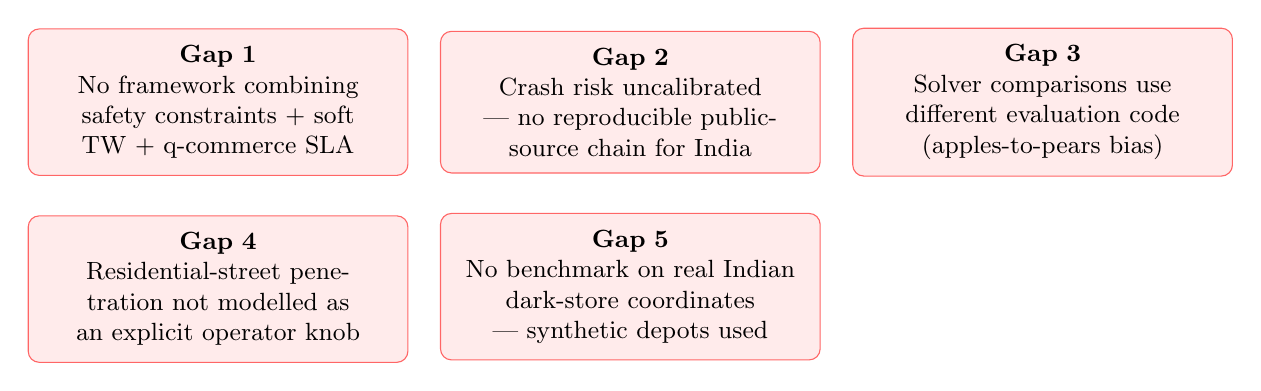
\begin{tikzpicture}[node distance=0.5cm and 0.3cm,
  gap/.style={draw=red!60,fill=red!8,rounded corners,text width=4.4cm,
              align=center,font=\small,inner sep=6pt,minimum height=1.4cm}]
\node[gap] (g1) {\textbf{Gap 1}\\No framework combining safety constraints + soft TW + q-commerce SLA};
\node[gap,right=0.4cm of g1] (g2) {\textbf{Gap 2}\\Crash risk uncalibrated --- no reproducible public-source chain for India};
\node[gap,right=0.4cm of g2] (g3) {\textbf{Gap 3}\\Solver comparisons use different evaluation code (apples-to-pears bias)};
\node[gap,below=0.5cm of g1] (g4) {\textbf{Gap 4}\\Residential-street penetration not modelled as an explicit operator knob};
\node[gap,below=0.5cm of g2] (g5) {\textbf{Gap 5}\\No benchmark on real Indian dark-store coordinates --- synthetic depots used};
\end{tikzpicture}
\end{center}
\vspace{6pt}
\begin{center}
  \textcolor{iitblue}{\Large$\Downarrow$}\\[3pt]
  \textbf{This thesis addresses all five gaps in one integrated, reproducible framework.}
\end{center}
\end{frame}

% Slide 5: Contributions
\begin{frame}{Contributions}
\begin{enumerate}
  \item \textbf{SA-VRPTW Formulation} --- crash exposure as hard
    $\varepsilon$-constraint ($\sum R_{ij}x_{ij}^k \leq \bar{R}$);
    per-route + fleet-wide residential caps $\bar{H}_k = 100$
  \item \textbf{BASM Calibration} --- reproducible public-source chain
    (MoRTH 2022 + Mohan et al.\ 2017 + OSM proxy) using only public data;
    explicit $\pi_{ij}$ formula published
  \item \textbf{Unified Solver Contract} --- MILP, GA, ALNS all share
    identical $F_1$ evaluation and feasibility checker
  \item \textbf{Key Empirical Finding} --- GA with BF-split outperforms
    ALNS at $N\geq100$ in quality AND speed (\textbf{325$\times$ faster at $N=200$})
  \item \textbf{Five-City Benchmark} --- real Blinkit dark-store coordinates
    (Bengaluru, Delhi, Gurugram, Mumbai, Pune); 428 feasible rows
  \item \textbf{Fully Reproducible Pipeline} --- Hydra config, seeded runs,
    manifest-checkpointed grid, MIT licence
\end{enumerate}
\end{frame}

% Slide 6: Problem Formulation
\begin{frame}{Problem Formulation: SA-VRPTW}
\begin{columns}[T]
\column{0.50\textwidth}
  \textbf{Primary Objective} (minimise service-quality cost):
  \[
    F_1 = \sum_{k}\sum_{i\in C}\!\Bigl[
      w_e\, w_i^k + \bigl(e^{\beta_{\text{stw}}\tau_i^k}-1\bigr)
    \Bigr]
  \]
  \begin{itemize}
    \item $w_i^k$: early-arrival idle wait
    \item $\tau_i^k$: lateness beyond 10-min ETA
    \item Convex penalty $\Rightarrow$ realistic SLA cost
  \end{itemize}
  \vspace{5pt}
  \textbf{$\varepsilon$-Constraints} (hard safety bounds):
  \begin{align*}
    &\textstyle\sum_{(i,j)} R_{ij}\,x_{ij}^k \leq \bar{R}
      \quad\forall k \;\;\text{(crash survival)}\\
    &\textstyle\sum_{(i,j)} H_{ij}\,x_{ij}^k \leq \bar{H}_k
      \quad\forall k \;\;\text{(residential cap)}\\
    &\textstyle\sum_k\sum_{(i,j)} H_{ij}\,x_{ij}^k \leq \bar{H}
      \;\;\text{(fleet-wide)}
  \end{align*}
\column{0.47\textwidth}
  \begin{block}{Super-Graph Arc Quantities}
    Shortest-time path $P_{uv}$ on street graph:
    \[
      T_{uv}=\!\sum_{e\in P}\! t_e,\;\;
      R_{uv}=\!\sum_{e}\!{-}\ln(1-r_e),\;\;
      H_{uv}=\!\sum_{e}\! h_e
    \]
  \end{block}
  \vspace{5pt}
  \begin{block}{Key Constants}
    \small
    \begin{tabular}{ll}
      $Q=2$ items & $T_{\max}=35$ min \\
      $\bar{H}_k=100$ edges & $\beta_{\text{stw}}=0.12$ \\
      PWL breakpoints: & $\{0,2,5,10,15,20,30\}$
    \end{tabular}
  \end{block}
  \vspace{4pt}
  {\footnotesize Multi-depot coupling, MTZ sub-tour elimination, and arrival-time linking constraints fully stated in Chapter 3.}
\end{columns}
\end{frame}

% Slide 7: Data Pipeline
\begin{frame}{Data Pipeline and BASM Calibration}
\begin{columns}[T]
\column{0.50\textwidth}
\begin{center}
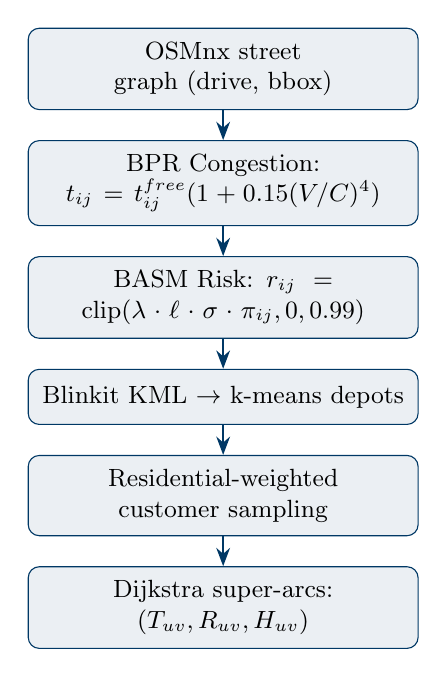
\begin{tikzpicture}[node distance=0.38cm,
  box/.style={draw=iitblue,fill=iitblue!8,rounded corners,
              text width=4.6cm,align=center,font=\small,
              inner sep=5pt,minimum height=0.7cm},
  arr/.style={-Stealth,thick,iitblue}]
  \node[box] (osm)  {OSMnx street graph (drive, bbox)};
  \node[box,below=of osm]  (bpr)  {BPR Congestion: $t_{ij}=t^{free}_{ij}(1+0.15(V/C)^4)$};
  \node[box,below=of bpr]  (basm) {BASM Risk: $r_{ij}=\mathrm{clip}(\lambda\cdot\ell\cdot\sigma\cdot\pi_{ij}, 0, 0.99)$};
  \node[box,below=of basm] (kml)  {Blinkit KML $\to$ k-means depots};
  \node[box,below=of kml]  (samp) {Residential-weighted customer sampling};
  \node[box,below=of samp] (arc)  {Dijkstra super-arcs: $(T_{uv}, R_{uv}, H_{uv})$};
  \draw[arr] (osm)--(bpr); \draw[arr] (bpr)--(basm);
  \draw[arr] (basm)--(kml); \draw[arr] (kml)--(samp);
  \draw[arr] (samp)--(arc);
\end{tikzpicture}
\end{center}
\column{0.47\textwidth}
  \textbf{BASM Local Proxy:}
  \[
    \pi_{ij} = \mathrm{clip}\!\bigl(
    1 + 0.40(2\beta_{ij}-1) + 0.30s_{ij} + 0.30c_{ij},\;
    0.5,\; 2.0\bigr)
  \]
  \begin{itemize}
    \item $\beta_{ij}$: normalised edge betweenness
    \item $s_{ij}$: local signal density
    \item $c_{ij}$: crossing density
  \end{itemize}
  \vspace{5pt}
  \textbf{Calibration chain:}
  \begin{itemize}
    \item MoRTH 2022 --- category-level fatality totals
    \item Mohan et al.\ 2017 --- arterial $>$ collector $>$ local
    \item OSM proxy --- \textbf{fully public, no restricted data needed}
  \end{itemize}
  \vspace{4pt}
  {\footnotesize Modelled annual events within $\pm25\%$ of city aggregate for all 5 cities.}
\end{columns}
\end{frame}

% Slide 8: Solver Architecture
\begin{frame}{Solver Architecture: Unified Evaluation Contract}
\begin{center}
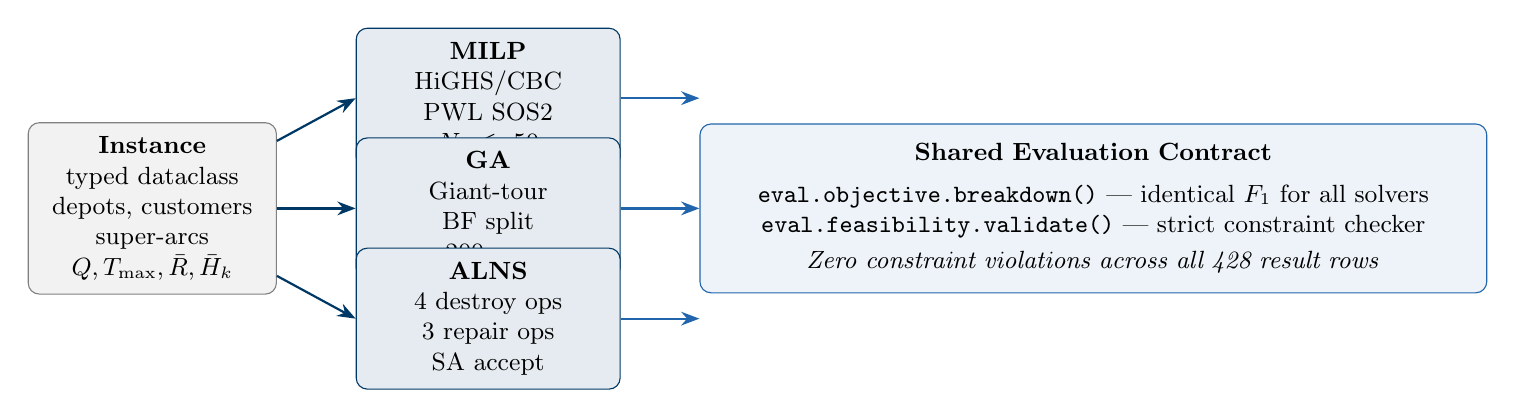
\begin{tikzpicture}[node distance=0.5cm and 0.7cm,
  solver/.style={draw=iitblue,fill=iitblue!10,rounded corners,
                 text width=3.0cm,align=center,font=\small,inner sep=5pt},
  contract/.style={draw=gacolor,fill=gacolor!8,rounded corners,
                   text width=9.5cm,align=center,font=\small,inner sep=7pt},
  inst/.style={draw=gray,fill=gray!10,rounded corners,
               text width=2.8cm,align=center,font=\small,inner sep=5pt},
  arr/.style={-Stealth,thick}]
  \node[inst] (inst) {\textbf{Instance}\\typed dataclass\\depots, customers\\super-arcs\\$Q,T_{\max},\bar{R},\bar{H}_k$};
  \node[solver,right=1.0cm of inst,yshift=1.4cm]  (milp) {\textbf{MILP}\\HiGHS/CBC\\PWL SOS2\\$N\leq50$};
  \node[solver,right=1.0cm of inst]               (ga)   {\textbf{GA}\\Giant-tour\\BF split\\200 gen};
  \node[solver,right=1.0cm of inst,yshift=-1.4cm] (alns) {\textbf{ALNS}\\4 destroy ops\\3 repair ops\\SA accept};
  \node[contract,right=1.0cm of ga] (eval)
    {\textbf{Shared Evaluation Contract}\\[4pt]
     \texttt{eval.objective.breakdown()} --- identical $F_1$ for all solvers\\
     \texttt{eval.feasibility.validate()} --- strict constraint checker\\[2pt]
     \textit{Zero constraint violations across all 428 result rows}};
  \draw[arr,iitblue] (inst) -- (milp.west);
  \draw[arr,iitblue] (inst) -- (ga.west);
  \draw[arr,iitblue] (inst) -- (alns.west);
  \draw[arr,gacolor] (milp.east) -- (eval.west|-milp.east);
  \draw[arr,gacolor] (ga.east)   -- (eval.west|-ga.east);
  \draw[arr,gacolor] (alns.east) -- (eval.west|-alns.east);
\end{tikzpicture}
\end{center}
\vspace{4pt}
\begin{columns}[T]
\column{0.32\textwidth}
  {\small\textbf{MILP}: exact benchmark; PWL outer-envelope for $e^{\beta\tau}-1$ via SOS2}
\column{0.34\textwidth}
  {\small\textbf{GA}: OX1 crossover; swap/insert/reverse mutation; BF split enforces hard caps}
\column{0.32\textwidth}
  {\small\textbf{ALNS}: Shaw/worst/random/risk-cluster destroy; greedy \& regret-2/3 repair}
\end{columns}
\end{frame}

% Slide 9: Algorithms
\begin{frame}{Algorithm Design: GA + ALNS Pseudocode}
\begin{columns}[T]
\column{0.48\textwidth}
  \begin{block}{Algorithm 1 --- GA with Bellman--Ford Split}
  \footnotesize
  \begin{tabbing}
  xx\=xx\=xx\=\kill
  \textbf{1.}\> Init $P$ random customer permutations\\
  \textbf{2.}\> Decode via BF split; evaluate $F_1$ + penalty\\
  \textbf{3.}\> \textbf{for} $g=1$ \textbf{to} $G=200$ \textbf{do}\\
  \textbf{4.}\>\> Carry top-$e=4$ elites forward\\
  \textbf{5.}\>\> $p_1,p_2 \leftarrow$ tournament($k=5$)\\
  \textbf{6.}\>\> Child $\leftarrow$ OX1 crossover ($p_x=0.85$)\\
  \textbf{7.}\>\> Apply swap / insert / reverse ($p_m=0.20$)\\
  \textbf{8.}\>\> Decode; evaluate; sort; truncate to $P$\\
  \textbf{9.}\> Validate incumbent via \texttt{validate()}\\
  \textbf{10.}\> \textbf{return} $s^*$
  \end{tabbing}
  \end{block}
  \vspace{4pt}
  {\footnotesize BF split adds $10^9$ sentinel for routes violating $H_k$, $\bar{R}$, or $T_{\max}$ --- hard constraints never silently broken.}
\column{0.48\textwidth}
  \begin{block}{Algorithm 2 --- ALNS}
  \footnotesize
  \begin{tabbing}
  xx\=xx\=xx\=\kill
  \textbf{1.}\> $s_0 \leftarrow$ GreedyConstruct($\mathcal{I}$)\\
  \textbf{2.}\> $T_{SA} \leftarrow 0.05\cdot F_1(s_0)$\\
  \textbf{3.}\> \textbf{for} $t=1$ \textbf{to} $5000$ \textbf{do}\\
  \textbf{4.}\>\> $q \leftarrow \lceil n\cdot U(0.15,0.45)\rceil$\\
  \textbf{5.}\>\> $D \leftarrow$ destroy op $\propto w^d$\\
  \textbf{6.}\>\> $R \leftarrow$ repair op $\propto w^r$\\
  \textbf{7.}\>\> $s' \leftarrow R(D(s,q))$\\
  \textbf{8.}\>\> Accept/reject via SA ($\eta=0.99975$)\\
  \textbf{9.}\>\> Update $\sigma=(33,9,1,0)$ weights\\
  \textbf{10.}\> Validate; \textbf{return} $s^*$
  \end{tabbing}
  \end{block}
  \vspace{4pt}
  {\footnotesize Destroy: random, worst-cost, Shaw relatedness, risk-cluster.\\
  Repair: greedy insert, regret-2, regret-3.}
\end{columns}
\end{frame}

% Slide 10: Code Snapshot
\begin{frame}[fragile]{Code Snapshot: Bellman--Ford Split with Hard-Constraint Sentinels}
\begin{columns}[T]
\column{0.58\textwidth}
\begin{lstlisting}
# src/savrptw/solvers/_common.py
HARD_VIOLATION = 1e9

for i in range(n):
    cumulative_load = 0
    for j in range(i + 1, n + 1):
        cumulative_load += customers[j-1].demand
        if cumulative_load > instance.Q:
            break  # capacity prune (O(n^2))

        rb = build_route(instance, depot,
                         customers[i:j],
                         penalty_weights=pw)
        # Soft F1 + penalty mass
        route_cost = rb.f1_contribution \
                   + rb.violation_mass

        # Hard-constraint sentinels
        if rb.total_H > instance.H_cap_route:
            route_cost += HARD_VIOLATION
        if rb.total_R > instance.R_bar:
            route_cost += HARD_VIOLATION
        if rb.duration > instance.T_max:
            route_cost += HARD_VIOLATION

        if cost[i] + route_cost < cost[j]:
            cost[j] = cost[i] + route_cost
            pred[j] = i
\end{lstlisting}
\column{0.39\textwidth}
  \vspace{4pt}
  \textbf{Why this design?}
  \begin{itemize}
    \item Shared by GA, ALNS, and MILP evaluator
    \item $F_1$ identical across all three --- no apples-to-pears bias
    \item $10^9$ sentinel: BF only selects a violating arc when \textit{no feasible split exists}
    \item $O(n^2)$ --- fast: 26 s at $N=200$
  \end{itemize}
  \vspace{6pt}
  \textbf{Project layout:}\\[3pt]
  {\footnotesize
  \texttt{src/savrptw/}\\
  \quad\texttt{solvers/} --- milp, ga, alns\\
  \quad\texttt{instance/} --- generator, super\_arc\\
  \quad\texttt{risk/} --- basm calibration\\
  \quad\texttt{eval/} --- feasibility, objective\\
  \texttt{conf/} --- Hydra YAML configs\\
  \texttt{scripts/} --- run\_grid.py
  }
\end{columns}
\end{frame}

% Slide 11: Experimental Setup
\begin{frame}{Experimental Setup}
\begin{columns}[T]
\column{0.48\textwidth}
  \textbf{Cities and Dark-Store Coverage}
  \begin{center}
  \small
  \begin{tabular}{lc}
  \toprule
  City & Blinkit stores \\
  \midrule
  Bengaluru & 113 \\
  Delhi     & 111 \\
  Mumbai    &  96 \\
  Gurugram  &  38 \\
  \midrule
  Pune      &  39 (partial data) \\
  Hyderabad &   0 (excluded) \\
  \bottomrule
  \end{tabular}
  \end{center}
  \vspace{4pt}
  \textbf{Grid:}
  \begin{itemize}
    \item $N \in \{20, 50, 100, 200\}$ customers
    \item Depots: $\{3, 5, 5, 8\}$ per $N$
    \item Up to 10 random seeds per cell
    \item Solvers: GA and ALNS
    \item \textbf{428 feasible rows}, 0 violations
  \end{itemize}
\column{0.48\textwidth}
  \begin{block}{Reproducibility}
    \begin{itemize}
      \item Hydra config composition
      \item Manifest-checkpointed grid runner --- crash-safe resumption
      \item All parameters in \texttt{conf/*.yaml}
      \item BASM guard: refuses uncalibrated source
    \end{itemize}
  \end{block}
  \vspace{5pt}
  \begin{block}{Evaluation}
    \begin{itemize}
      \item Strict \texttt{validate()} after every solve
      \item Crash Monte Carlo: 10,000 Bernoulli trials
      \item Beta-prior compliance sweep: $(\alpha,\beta)\in\{3,5,8\}\times\{1,2,3\}$
    \end{itemize}
  \end{block}
\end{columns}
\end{frame}

% Slide 12: Results F1 vs N
\begin{frame}{Results: $F_1$ vs Instance Size (All Cities)}
\begin{center}
  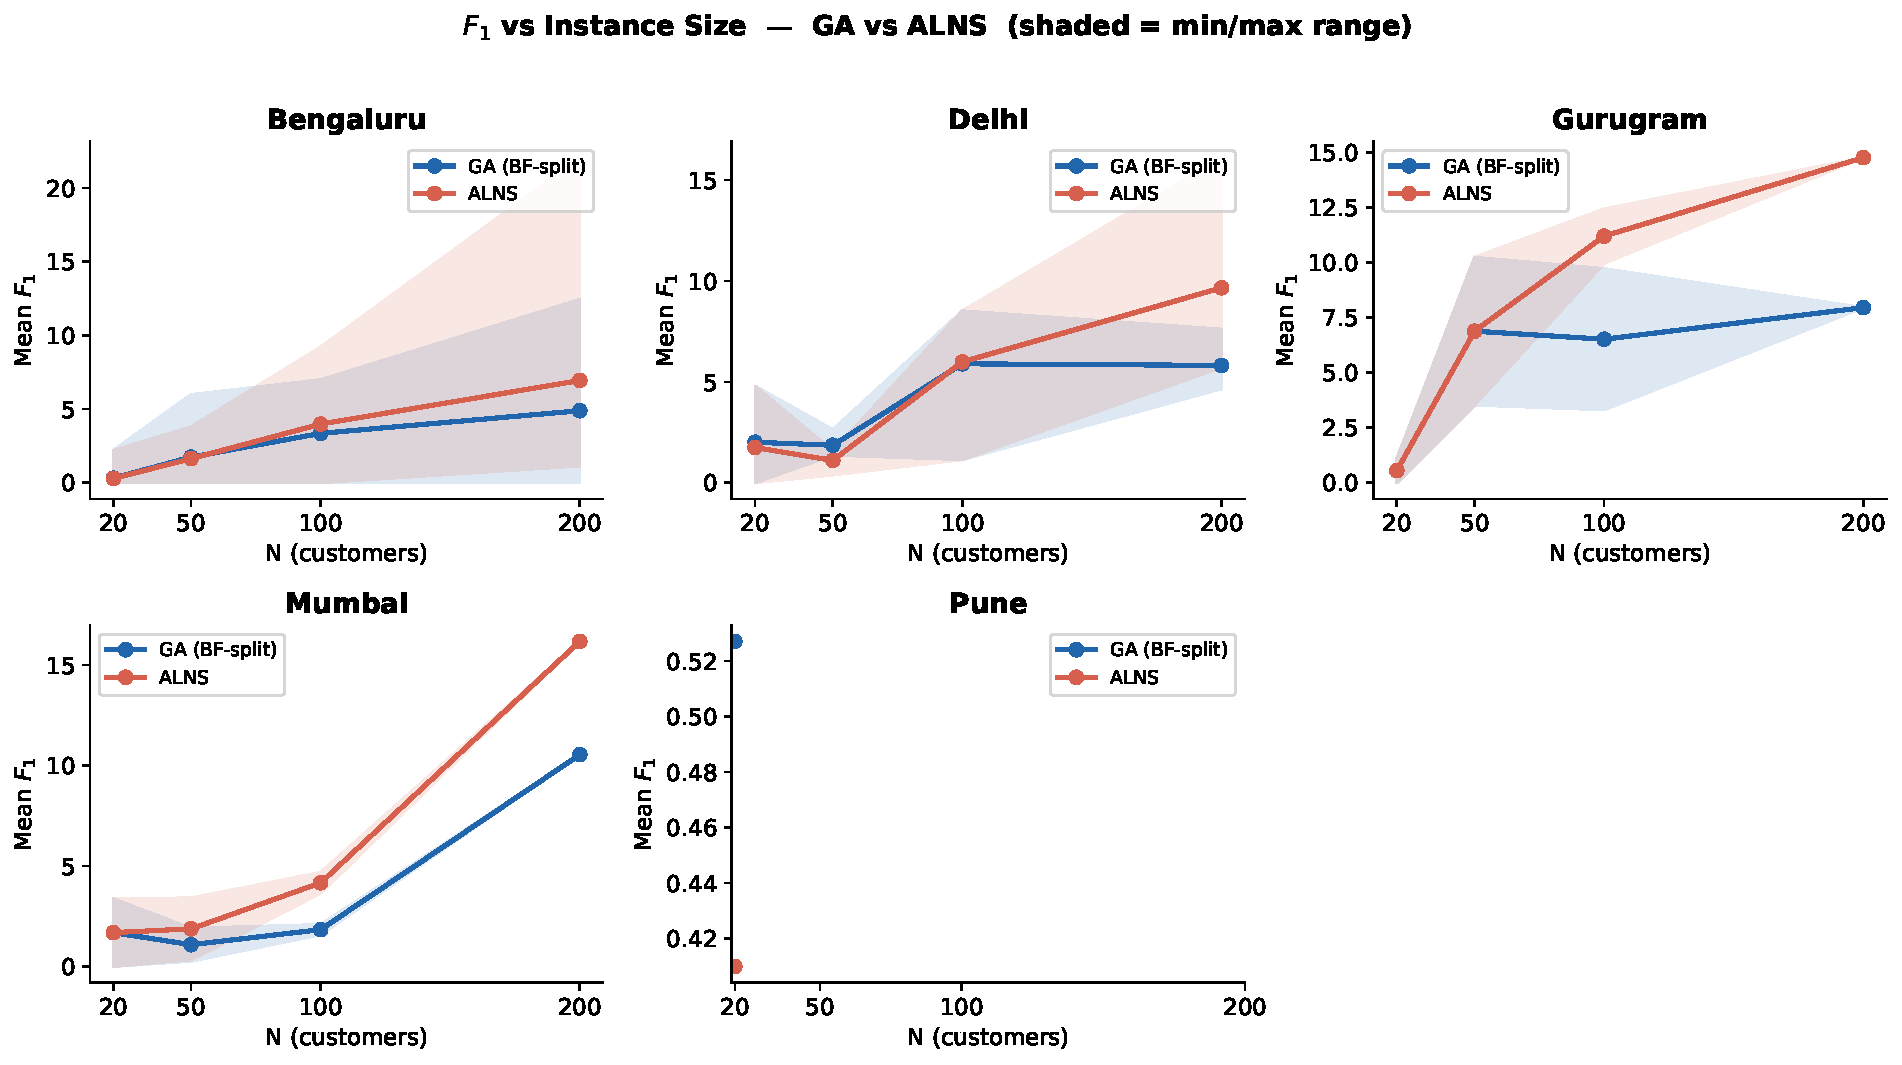
\includegraphics[width=0.88\textwidth]{../figures/fig_f1_vs_N.pdf}
\end{center}
\vspace{-4pt}
\begin{itemize}
  \item \textcolor{gacolor}{\textbf{GA}} and \textcolor{alnscolor}{\textbf{ALNS}}
        competitive at $N\leq50$; \textcolor{gacolor}{GA} clearly better at $N\geq100$
  \item $F_1$ grows near-linearly with $N$ for both solvers
  \item Wide bands at Gurugram and Delhi at $N=200$ --- seed-sensitive geometry
\end{itemize}
\end{frame}

% Slide 13: Results Wall-Clock and Speedup
\begin{frame}{Results: Wall-Clock Time and Speed-Up Ratio}
\begin{columns}[T]
\column{0.50\textwidth}
  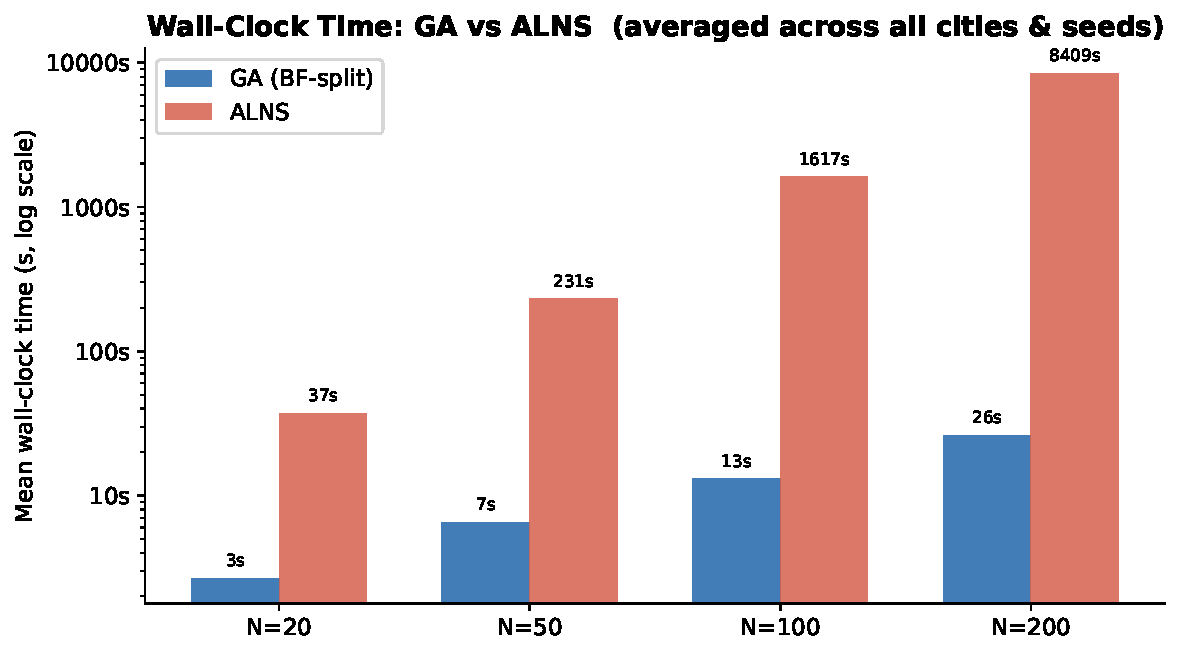
\includegraphics[width=\textwidth]{../figures/fig_wallclock.pdf}
\column{0.48\textwidth}
  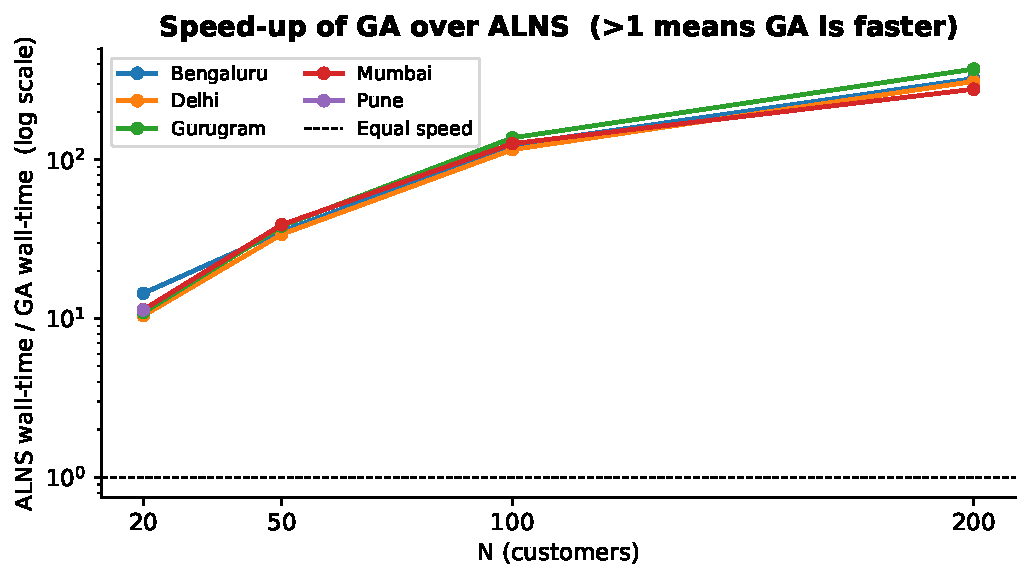
\includegraphics[width=\textwidth]{../figures/fig_speedup.pdf}
\end{columns}
\vspace{5pt}
\begin{center}
\begin{tabular}{lrrrr}
\toprule
Solver & $N=20$ & $N=50$ & $N=100$ & $N=200$ \\
\midrule
\textcolor{gacolor}{\textbf{GA}}     &  2.7 s &   6.5 s &    13 s &  \textbf{26 s} \\
\textcolor{alnscolor}{\textbf{ALNS}} &   31 s &   213 s &  1669 s & \textbf{8407 s} \\
\bottomrule
\end{tabular}
\end{center}
\vspace{2pt}
\begin{center}
\textcolor{iitblue}{\textbf{GA is $\sim$325$\times$ faster at $N=200$ and produces lower $F_1$}}
\end{center}
\end{frame}

% Slide 14: Results City Analysis
\begin{frame}{Results: City-Level Analysis}
\begin{columns}[T]
\column{0.52\textwidth}
  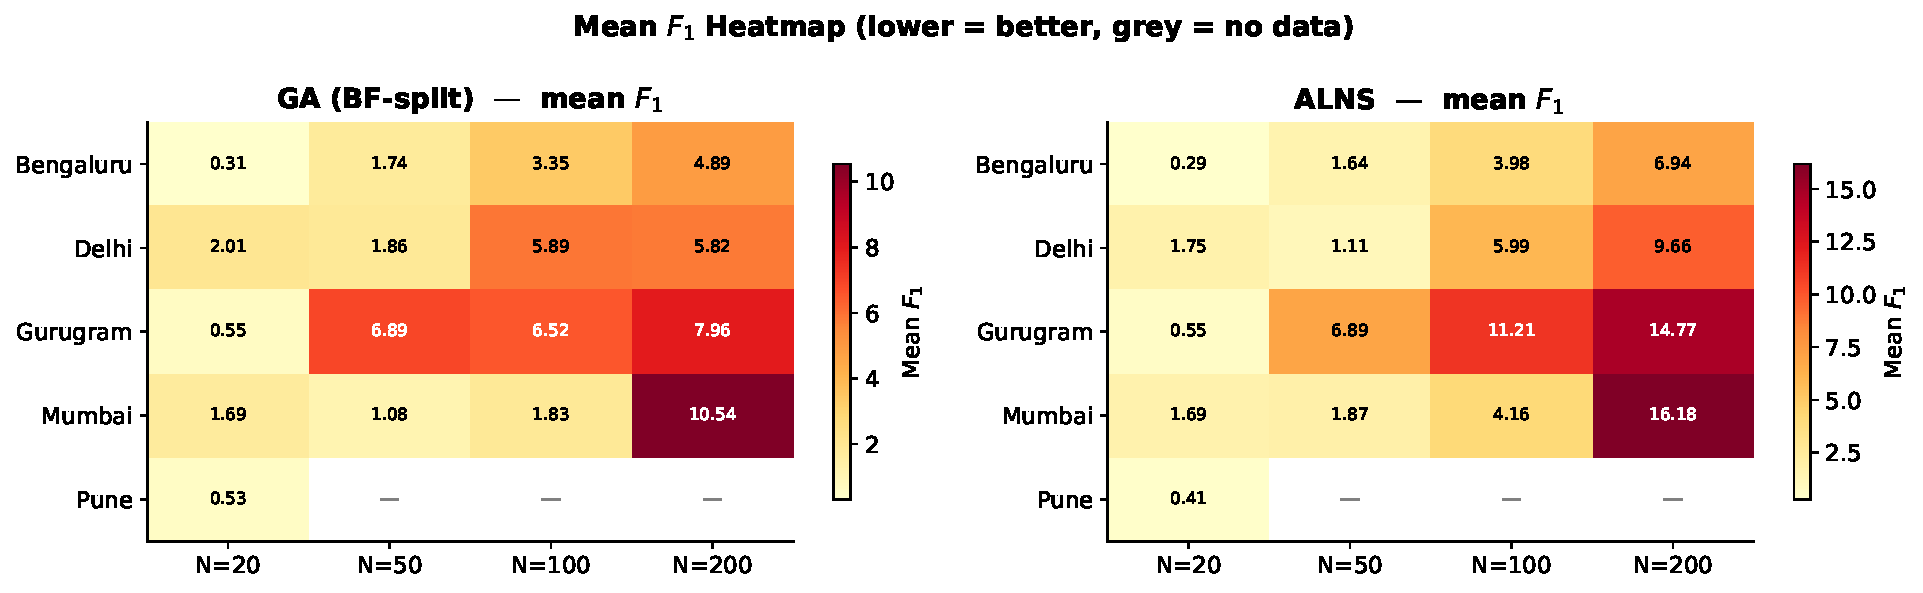
\includegraphics[width=\textwidth]{../figures/fig_heatmap_f1.pdf}
\column{0.46\textwidth}
  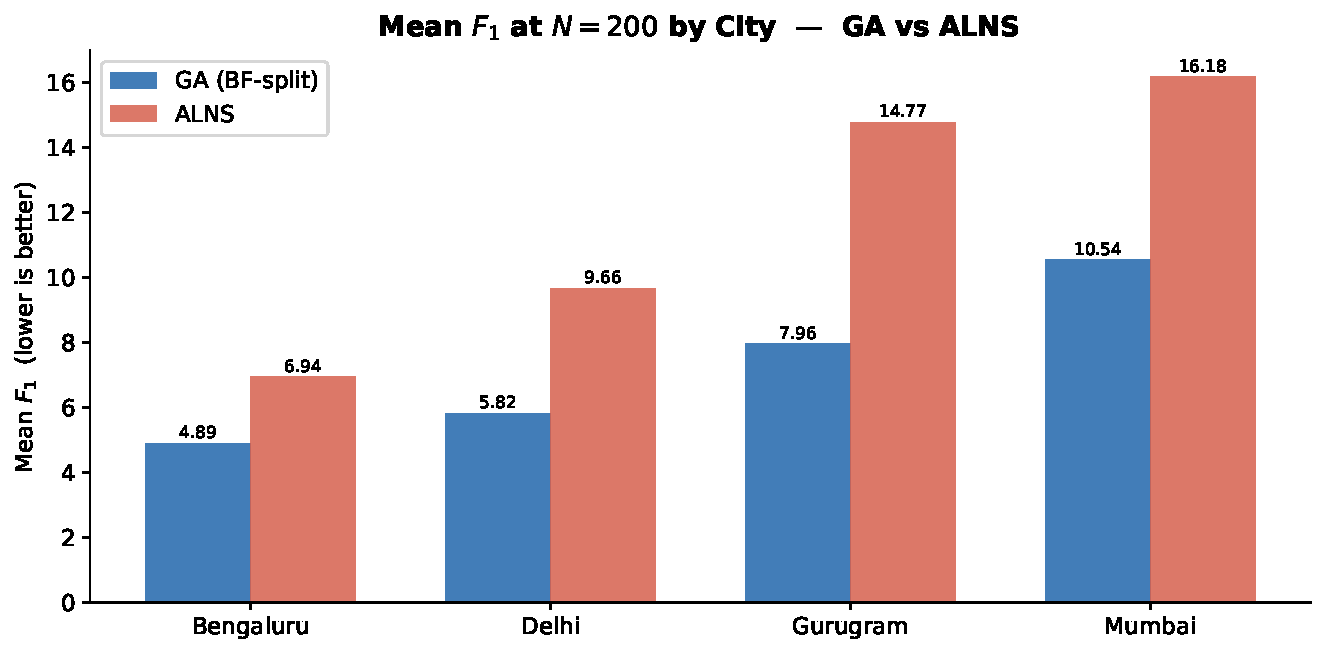
\includegraphics[width=\textwidth]{../figures/fig_f1_N200_cities.pdf}
\end{columns}
\vspace{4pt}
\begin{itemize}
  \item \textbf{Bengaluru} (113 stores) --- most stable; lowest $F_1$; recommended city for sensitivity studies
  \item \textbf{Gurugram \& Mumbai} --- elevated $F_1$ at $N\geq50$ due to fewer depot clusters relative to demand
  \item \textcolor{gacolor}{\textbf{GA}} consistently beats \textcolor{alnscolor}{\textbf{ALNS}} across all cities at $N=200$
  \item \textbf{Delhi} shows widest seed variance at large $N$ --- diverse street-network geometry
\end{itemize}
\end{frame}

% Slide 15: Limitations and Future Work
\begin{frame}{Limitations \& Future Work}
\begin{columns}[T]
\column{0.48\textwidth}
  \textbf{Honest Limitations}
  \begin{itemize}
    \item BASM is a \textit{calibrated prior}, not a direct measurement --- aggregate public data only
    \item Super-graph fixes paths: optimisation over customer
          \textbf{orderings}, not physical street choices
    \item MILP scales to $N\leq50$ only (CBC); commercial solver needed for larger
    \item Pareto $\bar{R}$--$\bar{H}$ sweep deferred to next run
    \item Behavioural compliance from single field-data study
  \end{itemize}
\column{0.48\textwidth}
  \textbf{Future Directions}
  \begin{enumerate}
    \item \textbf{Risk-aware path selection} --- jointly optimise orderings + physical streets
    \item \textbf{Pareto sweep} --- $\bar{R}\times\bar{H}$ grid traces safety/efficiency frontier
    \item \textbf{Real-time congestion} --- replace static BPR with live feeds
    \item \textbf{Stochastic demand} --- non-stationary order arrivals
    \item \textbf{Behavioural meta-analysis} --- multi-study compliance prior
    \item \textbf{City-level crash microdata} --- upgrade BASM with validated black-spot inventories if available
  \end{enumerate}
\end{columns}
\end{frame}

% Slide 16: Conclusion
\begin{frame}{Conclusion}
\begin{block}{What We Delivered}
  \begin{itemize}
    \item SA-VRPTW formulation with $\varepsilon$-constraints for crash survival and residential-road use
    \item Reproducible public-source BASM calibration for India --- no restricted data needed
    \item MILP, GA, and ALNS under a unified $F_1$/feasibility contract
    \item Empirical benchmark: 428 feasible rows, 5 cities, 4 problem sizes
  \end{itemize}
\end{block}
\vspace{5pt}
\begin{block}{Key Takeaways}
  \begin{itemize}
    \item \textbf{$\varepsilon$-constraint framing} gives operators an explicit safety dial --- no hidden weight tuning
    \item \textbf{GA with Bellman--Ford split} is recommended: \textit{both} faster and higher-quality than ALNS at $N\geq100$
    \item \textbf{Calibration honesty} is achievable without restricted microdata --- chain is fully reproducible
    \item Full pipeline released under \textbf{MIT licence}: \texttt{github.com/Coderopp/MTP-II}
  \end{itemize}
\end{block}
\end{frame}

% Slide 17: Thank You
\begin{frame}[plain]
\begin{center}
  \vspace{10pt}
  {\LARGE\textbf{Thank You}}\\[10pt]
  {\large Questions \& Discussion}\\[18pt]

  \begin{tabular}{rl}
    \textbf{Author:}      & Pranav Bhadane (21IM30017)\\
    \textbf{Supervisor:}  & Prof.\ Subhajit Sidhanta\\
    \textbf{Department:}  & Industrial \& Systems Engg., IIT Kharagpur\\
    \textbf{Code:}        & \texttt{github.com/Coderopp/MTP-II}\\
  \end{tabular}

  \vspace{14pt}
  \rule{0.55\textwidth}{0.4pt}\\[6pt]
  {\small
  \textit{Key references:}
  Solomon (1987) $\cdot$ Prins (2004) $\cdot$ Ropke \& Pisinger (2006)\\
  MoRTH (2022) $\cdot$ Mohan et al.\ (2017) $\cdot$ Boeing/OSMnx (2017)
  }
\end{center}
\end{frame}

\end{document}
